%空头
% UTF8编码,ctexart现实中文
%删除了\usepackage{color}
% 使用颜色
\definecolor{orange}{RGB}{255,127,0} 
\definecolor{violet}{RGB}{192,0,255} 
\definecolor{aqua}{RGB}{0,255,255} 
%删除了\usepackage{geometry}
\setcounter{tocdepth}{5}
\setcounter{secnumdepth}{5}
% 设置五级目录与标题
%删除A4
% 默认大小为A4
%删除页面边距
% 默认页边距为1英尺与1.25英尺
%删除了\usepackage{indentfirst}
%删除首行缩进
% 首行缩进2个中文字符
%删除\usepackage{setspace}
\renewcommand{\baselinestretch}{1.5}
% 1.5倍行距
%删除\usepackage{amssymb}
% 因为所以
%删除\usepackage{amsmath}
% 数学公式
%\usepackage[colorlinks,linkcolor=black,urlcolor=blue]{hyperref}
% 超链接
%\usepackage{tikz}
% 绘图

%删除了作者
\chapter{多元函数积分学}
%删除了页面格式
\section{二重积分}

\subsection{概念}

\subsubsection{几何背景}

二重积分的几何背景就是曲顶柱体的体积。定积分用极限的思想求出了二维平面的曲边梯形的面积,同样二重积分$\iint\limits_Df(x,y)\,\textrm{d}\sigma$。

被积函数$f(x,y)$作为曲顶柱体在点$(x,y)$处柱体微元的高,用底面积$\textrm{d}\sigma>0$乘上高$f(x,y)$就得到一个小柱体体积,再把所有$D$上的柱体相加起来就是整个曲顶柱体的体积。

\subsubsection{性质}

\begin{itemize}
    \item 求区域面积:$\iint\limits_D1\cdot\textrm{d}\sigma=\iint\limits_D\textrm{d}\sigma=A$,其中$A$为$D$的面积。
    \item 可积函数必有界:当$f(x,y)$在有界闭区间$D$上可积时,$f(x,y)$在$D$上必有界。
    \item 积分线性性质:$k_1,k_2$为常数,则$\iint\limits_D[k_1f(x,y)\pm k_2g(x,y)]\,\textrm{d}\sigma=$\\$k_1\iint\limits_Df(x,y)\,\textrm{d}\sigma\pm k_2\iint\limits_Df(x,y)\,\textrm{d}\sigma$。
    \item 积分可加性:当$f(x,y)$在有界闭区间$D$上可积时,且$D_1\cup D_2=D$,$D_1\cap U_2=\varnothing$,则$\iint\limits_Df(x,y)\,\textrm{d}\sigma=\iint\limits_{D_1}f(x,y)\,\textrm{d}\sigma+\iint\limits_{D_2}f(x,y)\,\textrm{d}\sigma$。
    \item 积分保号性:当$f(x,y),g(x,y))$在有界闭区间$D$上可积时,若在$D$上有$f(x,y)\leqslant g(x,y)$,则$\iint\limits_Df(x,y)\,\textrm{d}\sigma\leqslant\iint\limits_Dg(x,y)\,\textrm{d}\sigma$,特别$\left\vert\iint\limits_Df(x,y)\,\textrm{d}\sigma\right\vert\leqslant\iint\limits_D\vert f(x,y)\vert\,\textrm{d}\sigma$。
    \item 二重积分估值定理:设$M,m$,分别为$f(x,y)$在有界闭区域$D$上的最大值和最小值,$A$为$D$的面积,则有$mA\leqslant\iint\limits_Df(x,y)\,\textrm{d}\sigma\leqslant MA$。
    \item 二重积分中值定理:设函数$f(x,y)$在有界闭区域$D$上连续,$A$为$D$的面积,则在$D$上至少存在一点$(\xi,\eta)$使得$\iint\limits_Df(x,y)\,\textrm{d}\sigma=f(\xi,\eta)A$。
\end{itemize}

\textbf{例题:}设$I_1=\iint\limits_D\cos\sqrt{x^2+y^2}\,\textrm{d}\sigma$,$I_2=\iint\limits_D\cos(x^2+y^2)\,\textrm{d}\sigma$,$I_3=\iint\limits_D\cos(x^2+y^2)^2\,\textrm{d}\sigma$,其中$D=\{(x,y)|x^2+y^2\leqslant1\}$,则()。

$A.I_3>I_2>I_1$\qquad$B.I_1>I_2>I_3$\qquad$C.I_2>I_1>I_3$\qquad$D.I_3>I_1>I_2$

解:令$x^2+y^2=t$,$\therefore0<t\leqslant1$。所以$1\geqslant\sqrt{t}\geqslant t\geqslant t^2\geqslant0$。

又$\cos x$单调减,所以$A$。

\subsubsection{对称性}

普通对称性\textcolor{violet}{\textbf{定义:}}设$D$关于$y$轴对称,$I=\iint\limits_Df(x,y)\,\textrm{d}\sigma$,将$D$分为对称的两部分$D_1D_2$,即$I=\left\{\begin{array}{ll}
    2\iint\limits_{D_1}f(x,y)\,\textrm{d}\sigma, & f(x,y)=f(-x,y) \\
    0, & f(x,y)=-f(-x,y)
\end{array}\right.$。关于$x$轴对称也同理。

轮换对称性\textcolor{violet}{\textbf{定义:}}$xy$对调后区域$D$不变或关于$y=x$对称,$\iint\limits_Df(x,y)\,\textrm{d}x\textrm{d}y$\\$=\iint\limits_Df(y,x)\,\textrm{d}y\textrm{d}x$。类似积分值与积分变量无关。同理对于一元函数积分的不变性:$\int_a^bf(x)\,\textrm{d}x=\int_a^bf(y)\,\textrm{d}y$。

\textbf{例题:}设区域$D=\{(x,y)|x^2+y^2\leqslant1,x\geqslant0,y\geqslant0\}$,$f(x)$在$D$上的正值连续函数,$a,b$为常数,求$I=\displaystyle{\iint\limits_D\dfrac{a\sqrt{f(x)}+b\sqrt{f(y)}}{\sqrt{f(x)}+\sqrt{f(y)}}\textrm{d}\sigma}$。

解:由于被积函数是抽象的,所以无法直接计算。但是由于$D$是圆,$xy$对调后$D$保持不败你,所以$D$关于$y=x$对称,根据轮换对称性:\medskip

$I=\displaystyle{\iint\limits_D\dfrac{a\sqrt{f(x)}+b\sqrt{f(y)}}{\sqrt{f(x)}+\sqrt{f(y)}}\textrm{d}\sigma=\iint\limits_D\dfrac{a\sqrt{f(y)}+b\sqrt{f(x)}}{\sqrt{f(y)}+\sqrt{f(x)}}\textrm{d}\sigma}$。

$\therefore2I=\displaystyle{\iint\limits_D\dfrac{a\sqrt{f(x)}+b\sqrt{f(y)}}{\sqrt{f(x)}+\sqrt{f(y)}}\textrm{d}\sigma+\iint\limits_D\dfrac{a\sqrt{f(y)}+b\sqrt{f(x)}}{\sqrt{f(y)}+\sqrt{f(x)}}\textrm{d}\sigma}=\iint\limits_D(a+b)\,\textrm{d}\sigma$\\$=(a+b)\dfrac{\pi}{4}$。

解得$I=\dfrac{a+b}{8}\pi$。

\subsection{计算}

\subsubsection{直角坐标系}

后积先定限,先内画条线,先交写下限,后交写上限。

二重积分要将其变为累次积分,由一个区域的积分变为分别对$xy$的积分,要将$f(x,y)$拆开,重要的就是求上下限。

\paragraph{\texorpdfstring{$X$}型区域} \leavevmode \medskip

\begin{minipage}{0.6\linewidth}
    $\sigma=\{(x,y)|a\leqslant x\leqslant b,\psi(x)\leqslant y\leqslant\phi(x)\}$。
    
    也称为上下型区域。

    $\iint\limits_Df(x,y)\,\textrm{d}\sigma=\int_a^b\textrm{d}x\int_{\psi(x)}^{\phi(x)}f(x,y)\,\textrm{d}y$。
\end{minipage}
\hfill
\begin{minipage}{0.3\linewidth}
    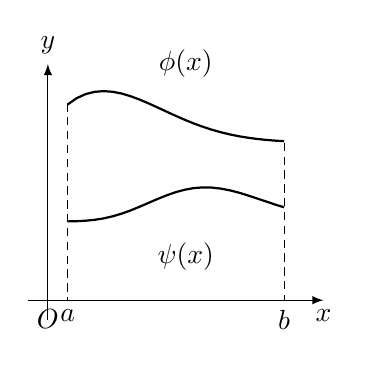
\begin{tikzpicture}[scale=1]
        \draw[-latex](-0.25,0) -- (3.5,0) node[below]{$x$};
        \draw[-latex](0,-0.25) -- (0,3) node[above]{$y$};
        \filldraw[black] (0,0) node[below]{$O$};
        \draw[black, thick, domain=0.25:3] plot (\x,{pow(\x,0.5)*pow(e,-\x*\x/2)+2});
        \filldraw[black] (1.75,3) node{$\phi(x)$};
        \draw[black, thick, domain=0.25:3] plot (\x,{pow(\x,4)*pow(e,-\x*\x/2)/5+1});
        \filldraw[black] (1.75,0.55) node{$\psi(x)$};
        \draw[black, densely dashed](0.25,2.5) -- (0.25,0) node[below]{$a$};
        \draw[black, densely dashed](3,2) -- (3,0) node[below]{$b$};
    \end{tikzpicture}
\end{minipage}

二重积分$X$型即求底部为如图的图形的面包状物体体积。求体积的做法就是已知截面面积求体积。其中横截面的一边在底面$\phi(x)-\psi(x)$,高为函数$f(x,y)$,则横截面面积$S(x)=\int^{\phi(x)}_{\psi(x)}f(x,y)\,\textrm{d}y$,得到了横截面之后再对$x$轴的所有横截面进行积分:$V=\int_a^bS(x)\,\textrm{d}x$就得到体积。

\paragraph{\texorpdfstring{$Y$}型区域} \leavevmode \medskip

\begin{minipage}{0.3\linewidth}
    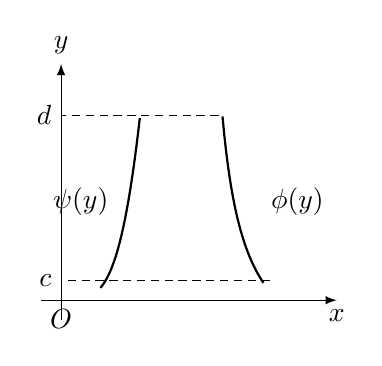
\begin{tikzpicture}[scale=1]
        \draw[-latex](-0.25,0) -- (3.5,0) node[below]{$x$};
        \draw[-latex](0,-0.25) -- (0,3) node[above]{$y$};
        \filldraw[black] (0,0) node[below]{$O$};
        \draw[black, thick, domain=2.05:2.57] plot (\x,{pow(\x-1.75,-1)-1});
        \filldraw[black] (3,1.25) node{$\phi(y)$};
        \draw[black, thick, domain=0.5:1] plot (\x,{pow(\x+0.25,6)*pow(e,-\x*\x/2)});
        \filldraw[black] (0.25,1.25) node{$\psi(y)$};
        \draw[black, densely dashed](2.65,0.25) -- (0,0.25) node[left]{$c$};
        \draw[black, densely dashed](2,2.35) -- (0,2.35) node[left]{$d$};
    \end{tikzpicture}
\end{minipage}
\hfill
\begin{minipage}{0.5\linewidth}
    $\sigma=\{(x,y)|c\leqslant x\leqslant d,\psi(y)\leqslant x\leqslant\phi(y)\}$。

    也称为左右型区域。

    $\iint\limits_Df(x,y)\,\textrm{d}\sigma=\int_c^d\textrm{d}y\int_{\psi(y)}^{\phi(y)}f(x,y)\,\textrm{d}x$。
\end{minipage}

\paragraph{区域类型选择} \leavevmode \medskip

若上下是两条曲线,那么就是$X$型,若左右是两条曲线,那么就是$Y$型。

若同一个方向的函数有两种不同的表达式,则从另一个方向将$D$按照函数分段割开求积分。

\subsubsection{极坐标系}

按积分区域与极点位置关系的不同,将二重积分计算分为三种情况:

根据$\theta$按角度切割区间,然后从极点开始按$\textrm{d}r$切割,变成一个个类似矩形的图形。图形一边为切割半径的改变量$\textrm{d}r$,另一条边为圆弧,等于半径乘改变角度$r\textrm{d}\theta$,所以最后$\textrm{d}\sigma=r\textrm{d}r\textrm{d}\theta$。

基本上都是先积$r$后积$\theta$。

从射线刚开始接触区域$D$的射线记为$\theta=\alpha$,要离开区域$D$的射线记为$\theta=\beta$,中间移动的射线为$\theta=\theta$。$\theta=\alpha$与$\theta=\beta$与$D$相交于两点,两点内靠近极点的$D$的边为\textbf{内曲线},远离极点的边为\textbf{外曲线}。$\theta=\theta$与内曲线交于$r=r_1(\theta)$,与外曲线交于$r=r_2(\theta)$。

\begin{enumerate}
    \item 极点$O$在区域$D$外部:$\iint\limits_Df(x,y)\,\textrm{d}\sigma=\int_\alpha^\beta\textrm{d}\theta\int_{r_1(\theta)}^{r_2(\theta)}f(r\cos\theta,r\sin\theta)r\,\textrm{d}r$。
    \item 极点$O$在区域$D$边上:$\iint\limits_Df(x,y)\,\textrm{d}\sigma=\int_\alpha^\beta\textrm{d}\theta\int_0^{r(\theta)}f(r\cos\theta,r\sin\theta)r\,\textrm{d}r$。
    \item 极点$O$在区域$D$内部:$\iint\limits_Df(x,y)\,\textrm{d}\sigma=\int_0^{2\pi}\textrm{d}\theta\int_0^{r(\theta)}f(r\cos\theta,r\sin\theta)r\,\textrm{d}r$。
\end{enumerate}

\subsubsection{极坐标系与直角坐标系选择}

若给出一个二重积分:

\begin{enumerate}
    \item 被积函数是否为$f(x^2+y^2)$、$f\left(\dfrac{y}{x}\right)$、$f\left(\dfrac{x}{y}\right)$等形式。
    \item 积分区域是否为圆或圆的一部分。
    \item 如果上面两种都有,则优先使用极坐标系,否则优先考虑直角坐标系。
\end{enumerate}

\subsubsection{极直互化}

对于极坐标系转换到直角坐标系:$x=r\cos\theta$,$y=r\sin\theta$。

\textbf{例题:}设区域$D=\{(x,y)|x^2+y^2\leqslant R^2\}$,计算$\displaystyle{\iint\limits_D\left(\dfrac{x^2}{a^2}+\dfrac{y^2}{b^2}\right)\textrm{d}x\textrm{d}y}$。

解:互换积分变量:$I=\displaystyle{\iint\limits_D\left(\dfrac{x^2}{a^2}+\dfrac{y^2}{b^2}\right)\textrm{d}x\textrm{d}y}=\displaystyle{\iint\limits_D\left(\dfrac{y^2}{a^2}+\dfrac{x^2}{b^2}\right)\textrm{d}x\textrm{d}y}$。

$\therefore2I=\left(\dfrac{1}{a^2}+\dfrac{1}{b^2}\right)\displaystyle{\iint\limits_D(x^2+y^2)\textrm{d}x\textrm{d}y}$,$\therefore I=\dfrac{1}{2}\left(\dfrac{1}{a^2}+\dfrac{1}{b^2}\right)\displaystyle{\iint\limits_D(x^2+y^2)\textrm{d}\sigma}$。

根据公式三转换为极坐标系:$I=\dfrac{1}{2}\left(\dfrac{1}{a^2}+\dfrac{1}{b^2}\right)\int_0^{2\pi}\textrm{d}\theta\int_0^Rr^2r\,\textrm{d}r$。

即$I=\left(\dfrac{1}{a^2}+\dfrac{1}{b^2}\right)\dfrac{\pi R^4}{4}$。

\textbf{例题:}计算$I=\int_0^1\textrm{d}x\int_{1-x}^{\sqrt{1-x^2}}\dfrac{x+y}{x^2+y^2}\textrm{d}y$。

解:根据上限$\sqrt{1-x^2}$和$1-x$所围成的图形$D$为第一象限的圆减去三角形。

所以转换为极坐标系时,对于$\theta\in\left(0,\dfrac{\pi}{2}\right)$,对于$r$在$(1-x,\sqrt{1-x^2})$。

下限$x+y=1$,即$r\cos\theta+r\sin\theta=1$,解出$r=\dfrac{1}{\cos\theta+\sin\theta}$,上限是一个圆,所以为1。

$=\int_0^\frac{\pi}{2}\textrm{d}\theta\int_\frac{1}{\cos\theta+\sin\theta}^1\cos\theta+\sin\theta\,\textrm{d}r=\int_0^\frac{\pi}{2}\cos\theta+\sin\theta-1\,\textrm{d}\theta=2-\dfrac{\pi}{2}$。

\subsubsection{积分次序}

积分次序即区域类型选择的问题,目的是为了简化计算,使得积分的函数更简单。

从另一方面,也很可能是积分函数无法按此次序进行积分,所以需要更换积分顺序。

存在许多有原函数但求不出初等函数形式的原函数。如$\dfrac{\sin x}{x}$、$\dfrac{\cos x}{x}$、$\dfrac{\tan x}{x}$、$\dfrac{e^x}{x}$、$\sin x^2$、$\cos x^2$、$\tan x^2$、$e^{ax^2+bx+c}$、$\dfrac{1}{\ln x}$等。

\textbf{例题:}计算$\displaystyle{\int_1^2\textrm{d}x\int_{\sqrt{x}}^x\sin\dfrac{\pi x}{2y}\textrm{d}y+\int_2^4\textrm{d}x\int_{\sqrt{x}}^2\sin\dfrac{\pi x}{2y}\textrm{d}y}$。

解:首先可以看出积分函数都是一样的,只是积分区域不同所以分开了,可见该函数的积分区域较复杂。

积分函数为$\sin\dfrac{\pi x}{2y}$,若对$y$进行积分,则可以类比求$\displaystyle{\int\sin\dfrac{1}{x}\,\textrm{d}x}$,这个是积分积不出来的。所以必须更换积分顺序。先积$x$。

首先根据被积函数上下限得到积分区域:$\sqrt{x}$、$x$、2围成的类三角形$\textrm{d}\sigma$。

$I=\displaystyle{\iint\limits_D\sin\dfrac{\pi x}{2y}\textrm{d}\sigma}=\displaystyle{\int_1^2\textrm{d}y\int_y^{y^2}\sin\dfrac{\pi x}{2y}\textrm{d}x}=\displaystyle{\int_1^2\dfrac{2y}{\pi}\left(-\cos\dfrac{\pi y}{2}+\cos\dfrac{\pi}{2}\right)}\textrm{d}y=\dfrac{4}{\pi^3}(2+\pi)$。

\subsubsection{二重积分处理一元积分}

在面对有中间变量的一元积分时,可以使用二重积分。

\textbf{例题:}设$f(x)=\int_x^1\sin(\pi u^2)\,\textrm{d}u$,求$\int_0^1f(x)\,\textrm{d}x$。(可以使用分部积分法)

解:$\int_0^1f(x)\,\textrm{d}x=\int_0^1\textrm{d}x\int_x^1\sin(\pi u^2)\,\textrm{d}u$。又$\sin(\pi u^2)$无法对$x$积分。

换做对$y$积分,$\textrm{d}\sigma$为$x=0$、$x=1$、$u=x$围成的三角形。交换积分次序:

$\int_0^1\textrm{d}y\int_0^u\sin(\pi u^2)\,\textrm{d}x=\int_0^1\sin(\pi u^2)u\,\textrm{d}u=\dfrac{1}{2\pi}\int_0^1\sin(\pi u^2)\,\textrm{d}(\pi u^2)=-\dfrac{1}{2\pi}$\\$\cos\pi u^2|_0^1=-\dfrac{1}{2\pi}(-1-1)=\dfrac{1}{\pi}$。

\textbf{例题:}利用广义二重积分求$\int_0^{+\infty}e^{-x^2}\,\textrm{d}x$。

解:根据积分值与积分变量无关的性质:

$I^2=(\int_0^{+\infty}e^{-x^2}\,\textrm{d}x)^2=\int_0^{+\infty}e^{-x^2}\,\textrm{d}x\cdot\int_0^{+\infty}e^{-y^2}\,\textrm{d}y=\int_0^{+\infty}\int_0^{+\infty}e^{-x^2-y^2}\,\textrm{d}x\textrm{d}y$

$\textrm{d}\sigma$是第一象限,可以看作一个广义的圆,半径无限大,转换为极坐标系。

$=\int_0^\frac{\pi}{2}\textrm{d}\theta\int_0^{+\infty}e^{-r^2}r\,\textrm{d}r=\displaystyle{\int_0^\frac{\pi}{2}\dfrac{1}{2}\,\textrm{d}\theta}=\dfrac{\pi}{2}$。$\therefore I=\dfrac{\sqrt{\pi}}{2}$。

\subsection{二重积分应用}

\subsubsection{体积}

\subsubsection{形心公式}

对于直角坐标系和参数方程:

$\overline{x}=\dfrac{\iint\limits_Dx\,\textrm{d}\sigma}{\iint\limits_D\textrm{d}\sigma}=\dfrac{\int x(t)y(t)x'(t)\,\textrm{d}t}{\int y(t)x'(t)\,\textrm{d}t}$,$\overline{y}=\dfrac{\iint\limits_Dy\,\textrm{d}\sigma}{\iint\limits_D\textrm{d}\sigma}=\dfrac{\int y(t)^tx'(t)\,\textrm{d}t}{\int y(t)x'(t)\,\textrm{d}t}$。

\section{三重积分}

\subsection{概念}

三重积分的被积函数$f(x,y,z)$定义在三维空间$\Omega$上,是四维空间图形体积,非常抽象。

所以利用质量描述,设一质量非均匀的物体,体积密度为$f(x,y,z)$,则三重积分就是以此为点密度的空间物体的质量。

\subsubsection{定义}

\textcolor{violet}{\textbf{定义:}}设三元函数$z=f(x,y,z)$定义在有界闭区域$\Omega$上将区域$\Omega$任意分成$n$个子域$\Delta v_i$($i=1,2,3,\cdots,n$)并以$\Delta v_i$表示第$i$个子域的体积。在$\Delta v_i$上任取一点$(\alpha_i,\beta_i,\gamma_i)$作和$\sum\limits_{i=1}^n\alpha_i\beta_i\gamma_i\Delta v_i$。如果当各个子域的直径中的最大值$\lambda$趋于零时,此和式的极限存在,则称此极限为函数$f(x,y,z)$在区域$\Omega$上的三重积分,记为$\iiint\limits_\Omega f(x,y,z)\,\textrm{d}v$,即$\iiint\limits_\Omega f(x,y,z)\,\textrm{d}v=\lim\limits_{\lambda\to0}\sum\limits_{i=1}^nf(x_i,y_i,z_i)\Delta y_i$,其中$\textrm{d}v$叫做体积元素。

其中$\iiint$称为三重积分号,$f(x,y,z)$为被积函数,$f(x,y,z)\textrm{d}v$称为被积表达式,$\textrm{d}v$称为体积元,$x$、$y$、$z$为积分变量,$\Omega$为积分区域,$\sum f(\alpha_i,\beta_i,\gamma_i)\Delta v_i$为积分和。

\subsubsection{性质}

假设$\Omega$为空间有界闭区域。

\begin{itemize}
    \item 空间区域体积:$\iiint\limits_\Omega1\,\textrm{d}v=\iiint\limits_\Omega\textrm{d}v=V$,其中$V$为$\Omega$的体积。
    \item 可积函数必有界:设$f(x,y,z)$在$\Omega$上可积,则在$\Omega$上必有界。
    \item 积分线性:设$k_1,k_2$为常数,则$\iiint\limits_\Omega[k_1f(x,y,z)\pm k_2g(x,y,z)]\textrm{d}v=k_1\iiint\limits_\Omega$\\$f(x,y,z)\,\textrm{d}v\pm k_2\iiint\limits_\Omega g(x,y,z)\,\textrm{d}v$。
    \item 积分可加性:设$f(x,y,z)$在$\Omega$上可积,且$\Omega_1\cup\Omega_2=\Omega$,$\Omega_1\cap\Omega_2=\varnothing$,则$\iiint\limits_\Omega f(x,y,z)\,\textrm{d}v=\iiint\limits_{\Omega_1}f(x,y,z)\,\textrm{d}v+\iiint\limits_{\Omega_2}f(x,y,z)\,\textrm{d}v$。
    \item 积分保号性:设$f(x,y,z)$,$g(x,y,z)$在$\Omega$上可积,且在$\Omega$上$f(x,y,z)\leqslant g(x,y,z)$,则有$\iiint\limits_\Omega f(x,y,z)\,\textrm{d}v\leqslant\iiint\limits_\Omega g(x,y,z)\,\textrm{d}v$。且利用不等式性质:$\vert\iiint\limits_\Omega f(x,y,z)\,\textrm{d}v\vert\leqslant\iiint\limits_\Omega\vert f(x,y,z)\vert\,\textrm{d}v$。
    \item 三重积分估值定理:设$M,m$分别为$f(x,y,z)$在$\Omega$上的最大值和最小值,$V$为$\Omega$的体积,则$mV\leqslant\iiint\limits_\Omega f(x,y,z)\,\textrm{d}v\leqslant MV$。
    \item 三种积分中值定理:设$f(x,y,z)$在$\Omega$上连续,$V$为$\Omega$的体积,则$\Omega$上至少存在一点$(\xi,\eta,\zeta)$使得$\iiint\limits_\Omega f(x,y,z)\,\textrm{d}v=f(\xi,\eta,\zeta)V$。
\end{itemize}

\subsubsection{对称性}

分析方法与二重积分完全一样。

\paragraph{普通对称性} \leavevmode \medskip

假设$\Omega$关于$yOz$面对称,则$\iiint\limits_\Omega f(x,y,z)\,\textrm{d}v=$\\$\left\{\begin{array}{ll}
    2\iiint\limits_{\Omega_1}f(x,y,z)\,\textrm{d}v, & f(x,y,z)=f(-x,y,z) \\
    0, & f(x,y,z)=-f(-x,y,z)
\end{array}\right.$,其中$\Omega_1$为$\Omega$在$yOz$面前面的部分。

\paragraph{轮换对称性} \leavevmode \medskip

若把$x$与$y$对调后,$\Omega$不变,则$\iiint\limits_\Omega f(x,y,z)\,\textrm{d}v=\iiint\limits_\Omega f(y,x,z)\,\textrm{d}v$,这就是\textbf{轮换对称性}。其他情况类似。

在使用轮换对称性的时候需要根据题目进行轮换,特别是根据所要求的被积函数$f(x)$,若$f(x)$中存在某些变量,则要将没有出现的变量换去。

\subsection{计算}

基本思想还是三重积分化为一重积分。

\subsubsection{基础方法}

\paragraph{直角坐标系} \leavevmode \medskip

即$\textrm{d}v=\textrm{d}x\textrm{d}y\textrm{d}z$,微元是一个长方体。

\subparagraph{先一后二法} \leavevmode \medskip

先$z$后$xy$,也称为投影穿线法。先做定积分后做二重积分。相当于对底面构造垂直于底面的线,将这个面上所有的线的体积积分起来就得到这个总体积,所以先一后二法要求底面是固定的微元。

适用场合:$\Omega$有下曲面$z=z_1(x,y)$、上曲面$z=z_2(x,y)$,无侧面或侧面为柱面。

如二重积分:后积先定限,限内画条线,先交写下限,后交写上限。

$\iiint\limits_\Omega f(x,y,z)\,\textrm{d}v=\iint\limits_{D_{xy}}\textrm{d}\sigma\int_{z_1(x,y)}^{z_2(x,y)}f(x,y,z)\,\textrm{d}z$。

\textbf{例题:}计算三重积分$I=\displaystyle{\iiint\limits_\Omega\dfrac{\textrm{d}x\textrm{d}y\textrm{d}z}{(1+x+y+z)^3}}$,其中$\Omega$是由平面$x=0,y=0,z=0$及$x+y+z=1$所围成的四面体。

解:根据图形,已知是一个四面体,所以下底面是一个1×1的等腰直角三角形$D_{xy}$,上曲面为一个等边三角形$z=-1-x-y$,有两个侧柱面。

则先将$I$消去$z$,再计算$xy$:$I=\displaystyle{\iint\limits_{D_{xy}}\textrm{d}\sigma\int_0^{1-x-y}\dfrac{1}{(1+x+y+z)^3}\textrm{d}z}$

$=\displaystyle{\iint\limits_{D_{xy}}\textrm{d}\sigma\left(-\dfrac{1}{2}\dfrac{1}{(1+x+y+z)^2}\bigg|_{z=0}^{z=1-x-y}\right)}=\displaystyle{\iint\limits_{D_{xy}}\dfrac{1}{2}\left(\dfrac{1}{(1+x+y)^2}-\dfrac{1}{4}\right)\,\textrm{d}\sigma}$\\$=\dfrac{1}{2}\int_0^1\textrm{d}x\int_0^{1-x}\left(\dfrac{1}{(1+x+y)^2}-\dfrac{1}{4}\right)\,\textrm{d}y=\dfrac{1}{2}\displaystyle{\int_0^1\left(-\dfrac{1}{4}x+\dfrac{1}{1+x}-\dfrac{1}{4}\right)\,\textrm{d}x}$\\$=\left(-\dfrac{1}{8}x^2+\ln(1+x)-\dfrac{1}{4}x\right)\bigg|_0^1=\dfrac{1}{2}\left(\ln2-\dfrac{5}{8}\right)$。

\subparagraph{先二后一法} \leavevmode \medskip

先$xy$后$z$,也称为定限截面法。先做二重积分后做定积分。相当于对体积进行平行于地面的切割为圆柱体,将所有在这个高上的圆柱体积分起来就得到这个总面积,所以先二后一要求高是固定的微元。

适用场合:$\Omega$是旋转体,上面和下面都是平面,中间为曲面,旋转曲面方程为$\Sigma:z=z(x,y)$。

后积先定限,限内截个面限。

$\iiint\limits_\Omega f(x,y,z)\,\textrm{d}v=\int\limits_a^b\textrm{d}z\iint\limits_{D_z}f(x,y,z)\,\textrm{d}\sigma$。

\paragraph{柱面坐标系} \leavevmode \medskip

若二重积分部分$\iint\limits_{D_{xy}}\textrm{d}\sigma$适用于极坐标系(即与圆相关),使用极坐标系表示,令$x=r\cos\theta$,$y=r\sin\theta$,便有$\iiint\limits_\Omega f(x,y,z)\,\textrm{d}x\textrm{d}y\textrm{d}z=\iiint\limits_\Omega f(r\cos\theta,r\sin\theta,z)r\,$\\$\textrm{d}r\textrm{d}\theta\textrm{d}z$。这就是柱面坐标系下三重积分的计算。

适用场合:被积函数含有$x^2+y^2$,积分区域为圆或部分圆。

即一个定积分加上一个极坐标系下的二重积分。

% 在直接坐标系的先二后一法,因为$\textrm{d}\sigma$是在与$z$相关的$D_z$区域,需要用$z$来表示函数,所以无法用两个变量来表示函数。

\textbf{例题:}计算$\iiint\limits_\Omega(x^2+y^2)\,\textrm{d}v$,其中$\Omega$是$\left\{\begin{array}{ll}
    y^2=2z \\
    x=0
\end{array}\right.$绕$z$轴旋转一周形成的曲面与平面$z=8$所围成的区域。

解:已知平面曲线绕$z$轴旋转,首先求这个旋转曲面。

首先令$P_1(x_1,y_1,z_1)$在该曲线上,即得到两个方程:$y_1^2=2z_1$,$x_1=0$。

取在旋转轴$z$轴上一点$P_0(0,0,0)$,对于纬圆上任一点$P(x,y,z)$,其中$\vert P_0P_1\vert=\vert PP_0\vert$,即$x_1^2+y_1^2+z_1^2=x^2+y^2+z^2$。

且向量$\overrightarrow{PP_1}$垂直于旋转轴$z$轴,所以$(x_1-x,y_1-y,z_1-z)\bot(0,0,1)$,$z_1-z=0$,$z_1=z$。

代入方程所以$x_1^2+y_1^2=x^2+y^2$,再代入$y_1^2=2z$,$x_1=0$,得到$2z=x^2+y^2$。

旋转曲面为$z=\dfrac{x^2+y^2}{2}$。且于$z=8$所得到一个旋转体。

因为选择体上下都是平面,侧面是曲面,所以使用先二后一法。其中$D:x^2+y^2\leqslant2z$。

$I=\int_0^8\textrm{d}z\iint\limits_D(x^2+y^2)\,\textrm{d}\sigma=\int_0^8\textrm{d}z\int_0^{2\pi}\textrm{d}\theta\int_0^{\sqrt{2z}}r^2r\,\textrm{d}r=\dfrac{1024}{3}\pi$。

\paragraph{球面坐标系} \leavevmode \medskip

\subparagraph{适用场合} \leavevmode \medskip

被积函数含有$x^2+y^2+z^2$或$x^2+y^2$,积分区域为球或球的部分,锥或锥的部分。

\subparagraph{原理} \leavevmode \medskip

利用三族面对$\Omega$进行切割:

\begin{enumerate}
    \item 首先用$r=r_0$从原点开始向外做球体进行切割,求半径为$r_0$,增量为$\textrm{d}r$。$r_0\in[0,+\infty)$。
    \item 然后用$\phi=\phi_0$从$z$轴为中心,原点为定点,做半顶角为$\phi_0$的圆锥面进行切割,增量为$\textrm{d}\phi$。$\phi_0\in[0,\pi]$。
    \item 最后用$\theta=\theta_0$以$z$为轴做半平面,与$xOz$夹角为$\theta_0$,增量为$\textrm{d}\theta$。$\theta\in[0,2\pi]$。
\end{enumerate}

首先在极坐标系中,弧长等于弧度乘半径,所以微元的由$\phi$确定的一边为$r\textrm{d}\phi$,对于$\theta$确定的一边,首先需要根据勾股定理得到弧长$r\sin\phi$,然后乘$\textrm{d}\theta$得到微元边长$r\sin\phi\textrm{d}\theta$,最后乘上$\textrm{d}r$,从而得到微元就是三边相乘:$r\textrm{d}\phi r\sin\phi\textrm{d}\theta\textrm{d}r$。

对$xyz$,由$\phi$推出的一个直角三角形的斜边为$r$,半顶角为$\phi$,所以$z$轴的直角边为$z=r\cos\phi$,又$x^2+y^2+z^2=r^2$,所以$x^2+y^2=r^2-z^2=r^2\sin^2\phi$,又$xOy$夹角为$\theta$,所以$x=r\sin\phi\cos\theta$,$y=r\sin\phi\sin\theta$。

\subparagraph{计算方法} \leavevmode \medskip

$\iiint\limits_\Omega f(x,y,z)\,\textrm{d}x\textrm{d}y\textrm{d}z=\iiint\limits_\Omega f(r\sin\phi\cos\theta,r\sin\phi\sin\theta,r\cos\phi)r^2\sin\phi\,\textrm{d}\theta\textrm{d}\phi\textrm{d}r$

令$x=r\cos\theta\sin\phi$、$y=r\sin\theta\sin\phi$、$z=r\cos\phi$,判断$xOy$面的与正方向夹角$\phi$,$xOz$面的与正方向夹角$\theta$。

\textbf{例题:}计算三重积分$\iiint\limits_\Omega(x^2+y^2)\,\textrm{d}v$,其中$\Omega$是半球面$x^2+y^2+z^2=a^2$($y\geqslant0$)与$xOz$面所围成的区域。

解:根据图形是一个右半球,所以$\theta$是$x$正轴到负轴一共$\pi$,$\phi$到正轴到负轴一共$\pi$,$r$从原点到最外面一共$a$。$f(x)=x^2+y^2=r^2\sin^2\phi$。

$\therefore I=\int_0^\pi\textrm{d}\theta\int_0^\pi\textrm{d}\phi\int_0^a(r^2\sin^2\phi)r^2\sin\phi\textrm{d}r$

\paragraph{对称性} \leavevmode \medskip

\subparagraph{普通对称性} \leavevmode \medskip

\textbf{例题:}计算$\iiint\limits_\Omega e^{\vert z\vert}\,\textrm{d}v$,其中$\Omega:x^2+y^2+z^2\leqslant1$。

解:已知$\Omega$为一个半径为1的球体。且球体球心在原点,利用普通对称性代入:$f(x,y,z)\,\textrm{d}v=e^{\vert z\vert}\,\textrm{d}v=\textrm{d}m=f(x,y,-z)\,\textrm{d}v=e^{\vert z\vert}\,\textrm{d}v=\textrm{d}m$,所以对于$f(x,y,z)$,在球体上下积分相同。

$\therefore\iiint\limits_\Omega e^{\vert z\vert}\,\textrm{d}v=2\iiint\limits_{\Omega_1}e^z\,\textrm{d}v$,其中$\Omega_1$为上半球体,即$\Omega_1:x^2+y^2+z^2\leqslant1,z\geqslant0$。

由于$f(x)=e^z$,只包含$z$的变量,所以使用先二后一法更简单。

由于截面是一个圆,所以令$z=z$,代入方程得到面积:$D:x^2+y^2\leqslant1-z^2$。所以这个圆的半径的平方就是$r^2=1-z^2$,面积为$\pi r^2=\pi(1-z^2)$。

$=2\int_0^1\textrm{d}z\iint\limits_De^z\,\textrm{d}\sigma=2\int_0^1e^z\cdot\pi(1-z^2)\,\textrm{d}z=2\pi$。

\subparagraph{轮换对称性} \leavevmode \medskip

\textbf{例题:}设$\Omega=\{(x,y,z)|x^2+y^2+z^2\leqslant1\}$,求$\iiint\limits_\Omega z^2\,\textrm{d}x\textrm{d}y\textrm{d}z$。

解:利用轮换对称性可知$\iiint\limits_\Omega x^2\,\textrm{d}x\textrm{d}y\textrm{d}z=\iiint\limits_\Omega y^2\,\textrm{d}x\textrm{d}y\textrm{d}z=\iiint\limits_\Omega z^2\,\textrm{d}x\textrm{d}y\textrm{d}z$。

$\therefore I=\dfrac{1}{3}\iiint\limits_\Omega(x^2+y^2+z^2)\,\textrm{d}x\textrm{d}y\textrm{d}z$。

\paragraph{形心公式逆用} \leavevmode \medskip

由$\overline{x}=\dfrac{\iiint\limits_\Omega x\,\textrm{d}v}{\iiint\limits_\Omega\textrm{d}v}$推出$\iiint\limits_\Omega x\,\textrm{d}v=\overline{x}\cdot V$,其中$V$是$\Omega$的体积。

\section{第一型曲线积分}

是由定积分推广而来。即对弧长曲线积分。

\subsection{概念}

用于计算密度不均匀的不规则形状细线质量。

\subsubsection{几何性质}

$L$是在$xOy$上的曲线段,$f(x,y)$在$L$上有界,将$L$分割为多个线段$\Delta S_1,\Delta S_2,\cdots,\Delta S_n$,假如取该线段某点$\forall(\xi_i,\eta_i)\in\Delta S_i$,则该线段的质量可以近似为$\Delta m_i\approx\rho(\xi_i,\eta_i)\Delta S_i$,所以整体线的质量$m\approx\sum\limits_{i=1}^n\rho(\xi_i,\eta_i)\Delta S_i$。$\lambda=\max\{\Delta S_1,\cdots,\Delta S_n\}$,若极限$m=\lim\limits_{\delta\to0}\sum\limits_{i=1}^n\rho(\xi_i,\eta_i)\Delta S_i$存在,称该极限为$f(x,y)$在$L$上对弧长的曲线积分$\int_Lf(x,y)\,\textrm{d}s$。

\subsubsection{定义}

第一类曲线积分为$\int_Lf(x,y)\,\textrm{d}s$。

\subsubsection{性质}

\begin{itemize}
    \item $\int_L1\,\textrm{d}s=l$。
    \item $\int_Lf(x,y)\,\textrm{d}s=\int_{L_1}f(x,y)\,\textrm{d}s+\int_{L_2}f(x,y)\,\textrm{d}s$。
    \item $\int_L(k_1f(x,y))\textrm{d}s\pm\int_L(k_2f(x,y))\textrm{d}s=k_1\int_Lf(x,y)\,\textrm{d}s\pm k_2\int_Lf(x,y)\textrm{d}s$。
\end{itemize}

\subsubsection{对称性}

\begin{itemize}
    \item $L$关于$y$轴对称,右边部分为$L_1$,若$f(-x,y)=-f(x,y)$,则$\int_Lf(x,y)\,\textrm{d}s=0$,若$f(-x,y)=f(x,y)$,则$\int_Lf(x,y)\,\textrm{d}s=2\int_{L_1}f(x,y)\,\textrm{d}s$。
    \item $L$关于$x$轴对称,上边部分为$L_1$,若$f(x,-y)=-f(x,y)$,则$\int_Lf(x,y)\,\textrm{d}s=0$,若$f(x,-y)=f(x,y)$,则$\int_Lf(x,y)\,\textrm{d}s=2\int_{L_1}f(x,y)\,\textrm{d}s$。
    \item $L$关于$y=x$对称,则$\int_Lf(x,y)\,\textrm{d}s=\int_Lf(x,y)\,\textrm{d}s$。
\end{itemize}

\subsection{计算}

\subsubsection{基础方法}

即化为定积分。一投(投影)二代(代入关系方程)三计算($\textrm{d}s$转换为$\textrm{d}x$等)。

\begin{itemize}
    \item $L:y=g(x)$($a\leqslant x\leqslant b$),$\int_Lf(x,y)\,\textrm{d}s=\int_a^bf[x,g(x)]\sqrt{1+g'^2(x)}\textrm{d}x$。
    \item $L:\left\{\begin{array}{c}
        x=\phi(t) \\
        y=\psi(t)
    \end{array}\right.$($\alpha\leqslant t\leqslant\beta$),$\int_Lf(x,y)\,\textrm{d}s=\int_\alpha^\beta f[\phi(t),\psi(t)]\\\sqrt{\phi'^2(t)+\psi'^2(t)}\textrm{d}t$。 
\end{itemize}

\paragraph{平面} \leavevmode \medskip

\textbf{例题:}计算$\oint\limits_\Gamma\vert y\vert\,\textrm{d}s$,其中$\Gamma$为球面$x^2+y^2+z^2=2$与平面$x=y$的交线。

解:根据普通对称性,对于$\vert y\vert$而言,其他象限的函数值都与第一象限区域的函数相等。令第一象限区域为$\Gamma_1$:

$\therefore\oint\limits_\Gamma\vert y\vert\,\textrm{d}s=4\oint\limits_{\Gamma_1}y\,\textrm{d}s$

根据交线方程进行联立,得到$x=\cos t$,$y=\cos t$,$z=\sqrt{2}\sin t$。

对于$\Gamma_1$,其角度为$t\in\left(0,\dfrac{\pi}{2}\right)$,$y=\cos t$。

又$\textrm{d}s=\sqrt{x_t'^2+y_t'^2+z_t'^2}$,所以$\textrm{d}t=\sqrt{2}\,\textrm{d}t$

$=4\int_0^\frac{\pi}{2}\cos t\sqrt{2}\,\textrm{d}t=4\sqrt{2}$。

\paragraph{空间} \leavevmode \medskip

\subsubsection{技术方法}

\paragraph{边界方程代入被积函数} \leavevmode \medskip

\paragraph{对称性} \leavevmode \medskip

\paragraph{形心公式逆用} \leavevmode \medskip

\section{第一型曲面积分}

$\textrm{d}s$为面微分。即对面积曲面积分。

\subsection{概念}

\subsubsection{几何性质}

若一块厚度不计的物体$\Sigma$在空间中,对$\Sigma$取面积微元$\forall\textrm{d}s\in\Sigma$,此时面积微元的面密度认定为均匀,其质量$\textrm{d}m=\rho(x,y,z)\textrm{d}s$。所以总质量$m=\iint_\Sigma\textrm{d}m=\iint_\Sigma\rho(x,y,z)\,\textrm{d}s$。

\subsubsection{定义}

$\iint_\Sigma f(x,y,z)\,\textrm{d}s$为$f(x,y,z)$在曲面$\Sigma$上的面积的曲面积分。

\subsubsection{性质}

\begin{itemize}
    \item $\iint_\Sigma1\,\textrm{d}s=\sigma$。
    \item $\Sigma$关于$xOy$对称,上部为$\Sigma_1$,如果$f(x,y,-z)=-f(x,y,z)$,则$\iint_\Sigma=0$,如果$f(x,y,-z)=f(x,y,z)$,则$\iint_\Sigma=2\iint_{\Sigma_1}$。
\end{itemize}

\subsection{计算}

\subsubsection{二重积分法}

还是一投二代三计算。

\begin{enumerate}
    \item 对$\Sigma$作图。
    \item 查看图形的奇偶性和对称性,如果对称则消去对应$x$、$y$、$z$的奇数次项。如果图形关于$xOy$对称,则出现$z$的奇数次项就去掉;同理关于$yOz$存在$x$的奇数次项就去掉,$xOz$存在$y$的奇数次项就去掉。
    \item 查看是否可以将题目中的常数项式子对$I$化简。
    \item 投影,如将$\Sigma$投影到$xOy$平面,$z=\psi(x,y)$,$(x,y)\in D_{xy}$。
    \item 求$\dfrac{\partial z}{\partial x}$、$\dfrac{\partial z}{\partial y}$,$\textrm{d}s=\sqrt{1+\left(\dfrac{\partial z}{\partial x}\right)^2+\left(\dfrac{\partial z}{\partial y}\right)^2}\textrm{d}\sigma$。
    \item 代入$\displaystyle{\iint\limits_\Sigma f(x,y,z)\,\textrm{d}s=\iint\limits_{D_{xy}}f[x,y,\psi(x,y)]\sqrt{1+\left(\dfrac{\partial z}{\partial x}\right)^2+\left(\dfrac{\partial z}{\partial y}\right)^2}\textrm{d}\sigma}$。
\end{enumerate}

\textbf{例题:}$I=\oiint_\Sigma(xy^2+z)\textrm{d}s$。$\Sigma:z=x^2+y^2,z\leqslant1$。

解:已知$\Sigma$是一个开口向$z$轴正方向的抛物面。不关于$z$轴对称,关于$x$轴和$y$轴对称。$I$中存在$x$的奇数次项$xy^2$则去掉,由于不存在$y$的奇数次项则跳过。

$\therefore I=\iint_\Sigma z\,\textrm{d}s$。所以$\Sigma$对$xOy$投影最好,为一个单位圆。

所以投影为单位圆$D_{xy}:x^2+y^2\leqslant1$。

$\dfrac{\partial z}{\partial x}=2x$,$\dfrac{\partial z}{\partial y}=2y$,$\textrm{d}s=\sqrt{1+4x^2+4y^2}\textrm{d}\sigma$。

$I=\iint_{D_{xy}}(x^2+y^2)\sqrt{1+4(x^2+y^2)}\,\textrm{d}\sigma=\int_0^2\pi\textrm{d}\theta\int_0^1r^3\sqrt{1+4r^2}\,\textrm{d}r=\\\pi\int_0^1r^2\sqrt{1+4r^2}\,\textrm{d}(r^2)$。

令$r^2=t$,$I=\pi\int_0^1t\sqrt{1+4t}\,\textrm{d}t$。令$\sqrt{1+4t}=u$,$=\pi\int_1^{\sqrt{5}}\dfrac{u^2-1}{4}u\dfrac{u}{2}\,\textrm{d}u=\dfrac{\pi}{8}\int_1^{\sqrt{5}}(u^4-u^2)\textrm{d}u=\dfrac{\pi}{8}(\dfrac{u^5}{5}-\dfrac{u^3}{3})\bigg\vert_1^{\sqrt{5}}=\dfrac{10}{3}\sqrt{5}+\dfrac{2}{15}$。

\textbf{例题:}设曲面$\Sigma:\vert x\vert+\vert y\vert+\vert z\vert=1$,求$\oiint_\Sigma(x+\vert y\vert)\,\textrm{d}s$。

解:曲面$\Sigma$是一个正八面体。又普通对称性得$\oiint\limits_\Sigma x\,\textrm{d}s=0$。

令第一卦限为$\Sigma_1$,所以根据普通对称性$\oiint\limits_\Sigma\vert y\vert\,\textrm{d}s=8\iint\limits_{\Sigma_1}y\,\textrm{d}s$

因为$x+y+z=1$和$\textrm{d}s=\sqrt{1+z_x'^2+z_y'^2}\,\textrm{d}x\textrm{d}y$交换$xy$保持不变。

根据轮换对称性$\iint\limits_{\Sigma_1}y\,\textrm{d}s=\iint\limits_{\Sigma_1}x\,\textrm{d}s$。

且对于$x+y+z=1$和用$xz$替换$y$(把微元曲面投到不同的坐标轴平面):$\textrm{d}s=\sqrt{1+y_x'^2+y_z'^2}\,\textrm{d}x\textrm{d}z$交换$xz$保持不变。

根据轮换对称性$\iint\limits_{\Sigma_1}y\,\textrm{d}s=\iint\limits_{\Sigma_1}x\,\textrm{d}s=\iint\limits_{\Sigma_1}z\,\textrm{d}s$。

$\therefore8\iint\limits_{\Sigma_1}y\,\textrm{d}s=\dfrac{8}{3}\iint\limits_{\Sigma_1}(x+y+z)\,\textrm{d}s=\dfrac{8}{3}\iint\limits_{\Sigma_1}\textrm{d}s=\dfrac{8}{3}S_{\Sigma_1}=\dfrac{8}{3}\dfrac{\sqrt{3}}{2}=\dfrac{4}{3}\sqrt{3}$。

\subsubsection{技术方法}

\paragraph{边界方程代入被积函数} \leavevmode \medskip

\paragraph{对称性} \leavevmode \medskip

\paragraph{形心公式逆用} \leavevmode \medskip

\section{多元积分应用}

包括二重积分、三重积分、一型曲线积分、一型曲面积分四个部分。

\subsection{几何量}

\subsubsection{平面区域}

\subsubsection{空间区域}

\subsubsection{空间曲线}

\subsubsection{空间曲面}

是考试的重点。

\subsection{重心与形心}

当密度$\rho$为一个固定常数时重心就是形心。

\subsubsection{平面薄片}

\subsubsection{空间物体}

是考试的重点。

\textbf{例题:}设空间物体$\Omega=\{(x,y,z)|x^2+y^2\leqslant z\leqslant1\}$,求$\Omega$的形心的竖坐标$\overline{z}$。

% 解:形心公式$\overline{z}=\dfrac{}{}$

\subsubsection{空间曲线}

\subsubsection{空间曲面}

\subsection{转动惯量}

可能会考到。

\subsubsection{平面薄片}

\subsubsection{空间物体}

\subsubsection{空间曲线}

\subsubsection{空间曲面}

\subsection{引力}

考的可能性很小。

\subsubsection{平面薄片}

\subsubsection{空间物体}

\subsubsection{空间曲线}

\subsubsection{空间曲面}

\section{第二型曲线积分}

第二型与第一型的差别就是第二型具有物理意义是有向的,而第一型具有几何意义是无向的。即对坐标曲线积分。

\subsection{概念}

\subsubsection{场的概念}

\textcolor{violet}{\textbf{定义:}}就是空间区域$\Omega$上的一种对应法则。

数量场就是对应数量没有方向。向量场就是有数量也有方向。

\subsubsection{几何性质}

对于双理想状态,对一个物体沿直线且均匀力道,则其功为$\vec{F}\cdot\overrightarrow{AB}$($\vec{F}$为力向量,$\overrightarrow{AB}$为物体移动向量)。

而对于双不理想状态,对一个物体沿曲线且变动力道做功,则无法得出结论。

令曲线为$L$,对$L$进行切分为微元$\forall\overrightarrow{\textrm{d}s}\in L$,则$\overrightarrow{\textrm{d}s}=\{\textrm{d}x,\textrm{d}y\}$。设变力$\vec{F}(x,y)=\{P(x,y),Q(x,y)\}$,则功的微元为$\textrm{d}\omega=\vec{F}\cdot\overrightarrow{\textrm{d}s}=P(x,y)\textrm{d}x+Q(x,y)\textrm{d}y$,所以对整体功进行积分$\omega=\int_L\textrm{d}\omega=\int_LP(x,y)\textrm{d}x+Q(x,y)\textrm{d}y$。

令曲线为$L$,对$L$进行切分为微元$\forall\overrightarrow{\textrm{d}s}\in L$,则$\overrightarrow{\textrm{d}s}=\{\textrm{d}x,\textrm{d}y,\textrm{d}z\}$。设变力$\vec{F}(x,y,z)=\{P(x,y,z),Q(x,y,z),R(x,y,z)\}$,则功的微元为$\textrm{d}\omega=\vec{F}\cdot\overrightarrow{\textrm{d}s}=P(x,y,z)\textrm{d}x+Q(x,y,z)\textrm{d}y+R(x,y,z)\textrm{d}z$,所以对整体功进行积分$\omega=\int_L\textrm{d}\omega=\int_LP(x,y,z)\textrm{d}x+Q(x,y,z)\textrm{d}y+R(x,y,z)\textrm{d}z$。

\subsubsection{定义}

对于二维,对坐标的曲线积分为$\int_LP(x,y)\textrm{d}x+Q(x,y)\textrm{d}y$,其中$\int_LP(x,y)\,\textrm{d}x$为$P(x,y)$在有向曲线段$L$上对坐标$x$求积分,$\int_LQ(x,y)\,\textrm{d}y$为$Q(x,y)$在有向曲线段$L$上对坐标$y$求积分。

对于三维,对坐标的曲线积分为$\int_LP(x,y,z)\textrm{d}x+Q(x,y,z)\textrm{d}y+R(x,y,z)\textrm{d}z$,同理如二维的定义。

\subsubsection{性质}

\begin{itemize}
    \item $\int_{L^-}P(x,y)\,\textrm{d}x+Q(x,y)\,\textrm{d}y=-\int_LP(x,y)\,\textrm{d}x+Q(x,y)\,\textrm{d}y$。
    \item $\int_LP(x,y)\,\textrm{d}x+Q(x,y)\,\textrm{d}y=\int_L(P(x,y)\cos\alpha+Q(x,y)\cos\beta)\textrm{d}s$。(利用方向余弦将第二类曲线积分化成第一类曲线积分)
\end{itemize}

\subsection{计算}

对于不封闭曲线使用定积分法,对于封闭曲线或封闭曲线部分使用二重积分法。

\subsubsection{定积分法}

由于第二类曲线积分积分值可正可负,所以只需要关心其起点$x=a$,其终点$x=b$。

\begin{itemize}
    \item $L:y=g(x)$($x$起于$x=a$终于$x=b$),$\int_LP(x,y)\,\textrm{d}x+Q(x,y)\,\textrm{d}y=\int_a^bP[x,g(x)]\,\textrm{d}x+Q[x,g(x)]g'(x)\,\textrm{d}x$。
    \item $L:\left\{\begin{array}{c}
        x=\phi(t) \\
        y=\psi(t)
    \end{array}\right.$($t$起于$\alpha$终于$\beta$),$\int_LP(x,y)\,\textrm{d}x+Q(x,y)\,\textrm{d}y=\\\int_\alpha^\beta P[\phi(t),\psi(t)]\phi'(t)\,\textrm{d}t+Q[\phi(t),\psi(t)]\psi'(t)\textrm{d}t$。 
\end{itemize}

\subsubsection{二重积分法}

是考试的重点,基本上都会考到,非常重要。

\paragraph{背景} \leavevmode \medskip

复平面上的一个区域$G$,如果在其中任做一条简单闭曲线,而闭曲线的内部总属于$G$,就称$G$为单连通区域。一个区域如果不是单连通区域,就称为多连通区域。即形象地说一块完整的凸图形即单连通,中间存在洞的或凹图形为多连通。

对于单连通区域,边界的正方向为逆时针方向,对于多连通区域,外边界的正方向是逆时针,内边界的正方向是顺时针。

在定积分中,使用牛顿-莱布尼茨公式,将$\int_a^bf(x)\,\textrm{d}x=F(b)-F(a)$,即将代表$[a,b]$范围积分域的积分值变为代表两点边界差值的函数值。在二重积分中,积分区域为一个连通域,其面积的积分就是二重积分,其周长的积分就是曲线积分,那么是否有这么一种方法,将域的关系转换为边界的关系,即是否存在一种方法将二重积分和曲线积分联系起来。

所以这个方法就是将曲线积分转换为二重积分,这个工具就是格林公式。

\paragraph{格林公式} \leavevmode \medskip

条件:

\begin{itemize}
    \item $D$为连通区域,$L$为$D$的正向边界。(如果$D$不是个完整的区域则添加线段,如果$L$为反向边界则添加负号)
    \item $P(x,y)$、$Q(x,y)$在$D$上连续可偏导。
\end{itemize}

$\displaystyle{\oint\limits_LP(x,y)\,\textrm{d}x+Q(x,y)\,\textrm{d}y=\iint\limits_D\left(\dfrac{\partial Q}{\partial x}-\dfrac{\partial P}{\partial y}\right)\textrm{d}\sigma}$。

\subsubsection{路径无关积分}

对于第二类曲线积分$\int_LP(x,y)\,\textrm{d}x+Q(x,y)\,\textrm{d}y$,其积分值可能与路径$L$相关,也可能与路径$L$无关。

若$D$为单连通区域,$P(x,y)$、$Q(x,y)$在$D$上连续可偏导,以下命题等价:

\begin{enumerate}
    \item $\int_LP(x,y)\,\textrm{d}x+Q(x,y)\,\textrm{d}y$与路径无关。
    \item $\forall C\in D$($C$为闭区域),$\oint_CP(x,y)\,\textrm{d}x+Q(x,y)\,\textrm{d}y=0$。
    \item 柯西黎曼条件:$\dfrac{\partial Q}{\partial x}\equiv\dfrac{\partial P}{\partial y}$。(最合适)
    \item $\exists u(x,y)$,使得$\textrm{d}u=P(x,y)\,\textrm{d}x+Q(x,y)\,\textrm{d}y$。即$\dfrac{\partial u}{\partial x}=P(x,y)$,$\dfrac{\partial u}{\partial y}=Q(x,y)$。
\end{enumerate}

则根据这些条件简化计算,若满足柯西黎曼条件:

\begin{enumerate}
    \item 求曲线积分:$\int_LP(x,y)\,\textrm{d}x+Q(x,y)\,\textrm{d}y=\int_{(x_0,y_0)}^{(x_1,y_1)}P(x,y)\,\textrm{d}x+Q(x,y)\,\textrm{d}y=\int_{x_0}^{x_1}P(x,y_0)\,\textrm{d}x+\int_{y_0}^{y_1}Q(x_1,y)\,\textrm{d}y$(先水平后垂直)。
    \item 能找到$u$,求曲线积分:有$\textrm{d}u=P(x,y)\,\textrm{d}x+Q(x,y)\,\textrm{d}y$,则$\int_LP(x,y)\,\textrm{d}x+Q(x,y)\,\textrm{d}y=\int_{(x_0,y_0)}^{(x_1,y_1)}\textrm{d}u=u(x_1,y_1)-u(x_0,y_0)$。
    \item 求全微分对应$u$表达式:则$u(x,y)=\int_{(x_0,y_0)}^{(x,y)}P(x,y)\,\textrm{d}x+Q(x,y)\,\textrm{d}y=\int_{x_0}^xP(x,y_0)\,\textrm{d}x+\int_{y_0}^yQ(x_1,y)\,\textrm{d}y$(先水平后垂直)。
\end{enumerate}

\textbf{例题:}已知$\psi(x)$可导,$\psi(0)=2$,$\int_Lxy^2\,\textrm{d}x+\psi(x)y\,\textrm{d}y$与路径无关,求$\psi(x)$,并计算$I=\int_{(1,2)}^{(2,3)}xy^2\,\textrm{d}x+\psi(x)y\,\textrm{d}y$。

解:已知$P=xy^2$,$y=\psi(x)y$。由于曲线积分与路径无关,所以$\dfrac{\partial Q}{\partial x}\equiv\dfrac{\partial P}{\partial y}$,所以$\psi'(x)y\equiv2xy$,$\psi'(x)=2x$,$\psi(x)=x^2+C$,又$\psi(0)=2$,$C=2$,$\psi(x)=x^2+2$。

所以$I=\int_{(1,2)}^{(2,3)}xy^2\,\textrm{d}x+(x^2+2)y\,\textrm{d}y$。

方法一:$I=\int_1^2x\cdot2^2\,\textrm{d}x+\int_2^3(2^2+2)y\,\textrm{d}y=2x^2\vert_1^2+3y^2\vert_2^3=6+15=21$。

方法二:$I=\int_{(1,2)}^{(2,3)}(xy^2\,\textrm{d}x+x^2y\,\textrm{d}y)+2y\,\textrm{d}y=\int_{(1,2)}^{(2,3)}\textrm{d}(\dfrac{1}{2}x^2y^2+y^2)=(\dfrac{1}{2}x^2y^2+y^2)|_{(1,2)}^{(2,3)}=27-6=21$。

\section{第二型曲面积分}

与第二型曲线积分一样,是有方向的。即对坐标曲面积分。

\subsection{概念}

\subsubsection{向量场的通量}

令一个不可压缩的向量场$\vec{v}=\{P,Q,R\}$,向量场中有一个面$\Sigma$,有不规则方向的流体流入或流出这个面,现在要求单位时间内流入指定侧的流量。

取一块有侧的面$\forall\overrightarrow{\textrm{d}s}\in\Sigma$,从$x$轴正方向部分将$\overrightarrow{\textrm{d}s}$向$yOz$面的投影记为$\textrm{d}y\textrm{d}z$。

当$\cos\alpha\geqslant0$即方向余弦非负的情况下,$\textrm{d}y\textrm{d}z=\textrm{d}s_{yOz}$即就等于投影面积;当$\cos\alpha<0$即方向余弦为负的情况下,$\textrm{d}y\textrm{d}z=-\textrm{d}s_{yOz}$即就等于负投影面积。实际上$\textrm{d}y\textrm{d}z=\textrm{d}s\cdot\cos\alpha$。同理其他两个方向也是如此。

所以对$\overrightarrow{\textrm{d}s}$进行三轴投影,得到$\overrightarrow{\textrm{d}s}=\{\textrm{d}y\textrm{d}z,\textrm{d}z\textrm{d}x,\textrm{d}x\textrm{d}y\}$

所以$\overrightarrow{\textrm{d}s}$单位时间内流入指定侧的流量$\textrm{d}\phi=\vec{v}\cdot\overrightarrow{\textrm{d}s}=P(x,y,z)\textrm{d}y\textrm{d}z+Q(x,y,z)\textrm{d}z\textrm{d}x+R(x,y,z)\textrm{d}x\textrm{d}y$。

从而总流量为$\iint_\Sigma\textrm{d}\phi=\iint_\Sigma P(x,y,z)\textrm{d}y\textrm{d}z+Q(x,y,z)\textrm{d}z\textrm{d}x+R(x,y,z)\textrm{d}x\textrm{d}y$。

\subsubsection{定义}

$\iint_\Sigma P(x,y,z)\textrm{d}y\textrm{d}z+Q(x,y,z)\textrm{d}z\textrm{d}x+R(x,y,z)\textrm{d}x\textrm{d}y$为在$\Sigma$上的曲面积分。其中$\iint_\Sigma P(x,y,z)\textrm{d}y\textrm{d}z$为$P(x,y,z)$在有侧曲面$\Sigma$上对坐标$y$、$z$的曲面积分。

\subsubsection{性质}

\begin{itemize}
    \item $\iint_{\Sigma^-}=-\iint_\Sigma$。
    \item $\iint_\Sigma P(x,y,z)\textrm{d}y\textrm{d}z+Q(x,y,z)\textrm{d}z\textrm{d}x+R(x,y,z)\textrm{d}x\textrm{d}y=\iint_\Sigma P(x,y,z)\cos\alpha+Q(x,y,z)\cos\beta+R(x,y,z)\cos\gamma$。(曲面积分转为曲线积分)
    \item 若积分曲面对称:被积函数关于相应变量为奇函数,积分为半区间的2倍;若为偶函数,则积分等于0。(与一般奇偶性正好相反)
\end{itemize}

对于奇偶性的解释:因为是第二型的曲面积分,会分前后左右上下,分别代表正负,所以被积函数为偶函数时如果是相反方向,就正好被减去了(两个积的结果相同,方向相反,可以考虑磁通量一边进,一边出),奇函数两边想减因为方向不同,所以--为正相加,即为两倍。第一型曲面积分物理意义来源于对给定密度函数的空间曲面,计算该曲面的质量。第二型曲面积分物理意义来源对于给定的空间曲面和流体的流速,计算单位时间流经曲面的总流量。

\subsection{计算}

\subsubsection{二重积分法}

曲面积分的二重积分法较复杂。将积分化为不同面的投影。为什么会带一个正负号?因为前面的$\textrm{d}x\textrm{d}y\textrm{d}z$表示投影,其值可正可负,而后面的$\textrm{d}x\textrm{d}y\textrm{d}z$表示面积,必然为正。

\begin{itemize}
    \item $\oiint_\Sigma P(x,y,z)\,\textrm{d}y\textrm{d}z$:用$yz$表示$x$:$\Sigma:x=\phi(y,z)$,$(y,z)\in D_{yz}$,\\$\iint_\Sigma P(x,y,z)\,\textrm{d}y\textrm{d}z=\pm\iint_{D_{yz}}P[\phi(y,z),y,z]\textrm{d}y\textrm{d}z$。前正后负。
    \item $\oiint_\Sigma Q(x,y,z)\,\textrm{d}z\textrm{d}x$:用$xz$表示$y$:$\Sigma:y=\phi(z,x)$,$(z,x)\in D_{zx}$,\\$\iint_\Sigma Q(x,y,z)\,\textrm{d}z\textrm{d}x=\pm\iint_{D_{zx}}Q[x,\phi(z,x),z]\textrm{d}z\textrm{d}x$。右正左负。
    \item $\oiint_\Sigma R(x,y,z)\,\textrm{d}x\textrm{d}y$:用$xy$表示$z$:$\Sigma:z=\phi(x,y)$,$(x,y)\in D_{xy}$,\\$\iint_\Sigma R(x,y,z)\,\textrm{d}x\textrm{d}y=\pm\iint_{D_{xy}}R[x,y,\phi(x,y)]\textrm{d}x\textrm{d}y$。上正下负。
\end{itemize}

\subsubsection{三重积分法}

是考试的重点,基本上都会考到。非常重要。

\paragraph{背景} \leavevmode \medskip

牛顿莱布尼兹公式将定积分转换为函数值差,格林公式将曲线积分转换为二重积分,高斯公式就是将曲面积分转换为三重积分。

\paragraph{高斯公式} \leavevmode \medskip

条件:

\begin{itemize}
    \item $\Omega$为几何体,$\Sigma$为$\Omega$的外表面。(如果不封闭则补全,如果是内表面就添加负号)
    \item $P(x,y,z)$、$Q(x,y,z)$、$R(x,y,z)$在$\Omega$上连续可偏导。
\end{itemize}

$\displaystyle{\oiint_\Sigma P\,\textrm{d}y\textrm{d}z+Q\,\textrm{d}z\textrm{d}x+R\,\textrm{d}x\textrm{d}y=\iiint\limits_\Omega\left(\dfrac{\partial P}{\partial x}+\dfrac{\partial Q}{\partial y}+\dfrac{\partial R}{\partial z}\right)\textrm{d}v}$。

\textbf{例题:}$I=\iint_\Sigma yz\,\textrm{d}z\textrm{d}x+2\,\textrm{d}x\textrm{d}y$,其中$\Sigma$为$x^2+y^2+z^2=4$的$xOy$面的上半部分。

解:由$I$可得$P=0$,$Q=yz$,$R=2$,$\dfrac{\partial P}{\partial x}=0$,$\dfrac{\partial Q}{\partial y}=z$,$\dfrac{\partial R}{\partial z}=0$。

由于$\Sigma$只有球面的上半部分,所以需要补充底面$\Sigma_0:y=0$($x^2+y^2\leqslant4$下侧),此时才是一个半球体的完整封闭表面积,$\Sigma_0$的法向量为$z$轴的反方向。所以$I=\oiint_{\Sigma+\Sigma_0}-\iint_{\Sigma_0}$。

又根据高斯公式$\oiint_{\Sigma+\Sigma_0}=\iiint_\Omega z\,\textrm{d}v=\int_0^{2\pi}\textrm{d}\theta\int_0^{\frac{\pi}{2}}\textrm{d}\psi\int_0^2r\cos\psi\cdot r^2\sin\psi\,\textrm{d}r=2\pi\int_0^{\frac{\pi}{2}}\sin\psi\,\textrm{d}(\sin\psi)\int_0^2r^3\,\textrm{d}r=2\pi\times\dfrac{1}{2}\sin^2\psi\vert_0^{\frac{\pi}{2}}\times\dfrac{r^4}{4}\vert_0^2=4\pi$。

而底面$\iint_{\Sigma_0}yz\,\textrm{d}z\textrm{d}x+2\,\textrm{d}x\textrm{d}y=\iint_{\Sigma_0}2\,\textrm{d}x\textrm{d}y=-2\iint_{D_{xy}}\textrm{d}x\textrm{d}y=-8\pi$。

$I=4\pi+8\pi=12\pi$。

\section{空间第二型曲线积分计算}

是第二型曲线积分的应用。使用的是斯托克斯公式。

%\end{document}
